\section{Struttura del progetto}
Tutto il progetto è strutturato in 3 \emph{package(Domino,Task,Utility)}.
Nel corso della descrizione del codice, assumeremo che il lettore possieda già basi del linguaggio di programmazione \emph{Java}. Per cui, sarà omessa la differenziazione tra metodi pubblici, metodi privati e metodi statici delle singole classi.

\begin{figure}[H]
	\centering
	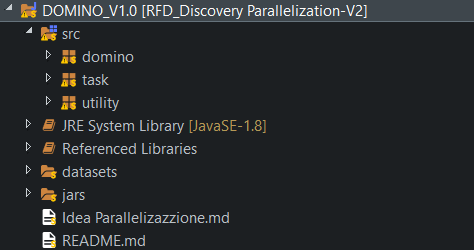
\includegraphics{Immagini/StrutturaProgetto.png}
	\caption{Struttura del Progetto}
	\label{fig:StrutturaProgetto}
\end{figure}

\subsection{Package Domino}
Il contenuto di questo pacchetto è costituito dalle principali classi che compongono la logica dell'algoritmo. Particolare enfasi è stata sottoposta alla classe \textbf{Domino.java}.
\begin{figure}[H]
	\centering
	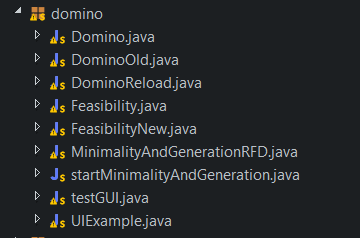
\includegraphics{Immagini/PackageRFD.png}
	\caption{Package Domino}
	\label{fig:Package Domino}
\end{figure}
Quest'ultima ha il compito di parallelizzare la fase di \textbf{Feasibility} e \textbf{Minimality}.
In particolare per ogni candidato \textbf{RHS} viene associato all'executor un \textbf{FeasibilityTask}.
Una volta ottenuti gli \textbf{insiemiC}, ognuno di essi verrà associato al rispettivo \textbf{MinimalityTask}. Ottenuto l'output dai task si procede alla ricombinazione di essi all'interno della \textbf{listaCC}.

\begin{figure}[H]
	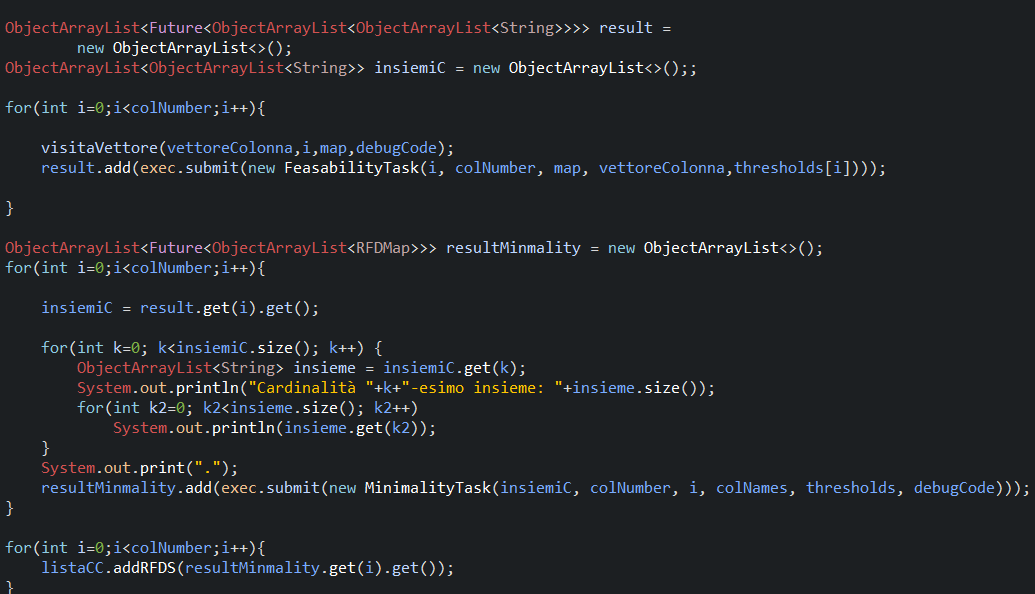
\includegraphics[scale=0.70]{Immagini/Executor.PNG}
	\caption{Codice Executor}
	\label{fig:Codice Executor}
\end{figure}

\subsection{Package Task}
Il contenuto di questo pacchetto è costituito dalle classi implementate per l'utilizzo dei task.
\begin{figure}[H]
	\centering
	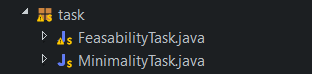
\includegraphics{Immagini/PackageTask.PNG}
	\caption{Package Task}
	\label{fig:Package Task}
\end{figure}
\subsubsection{FeasibilityTask}
\begin{figure}[H]
	\centering
	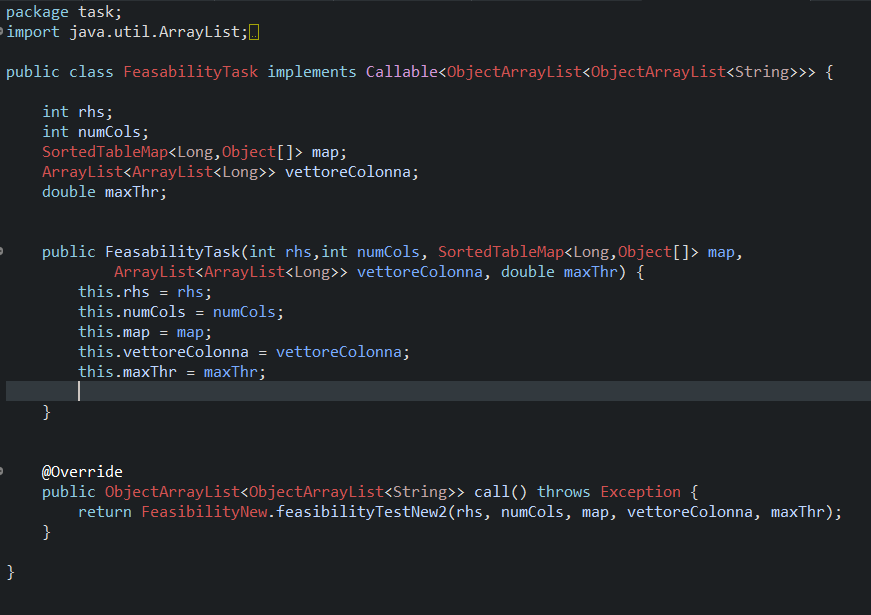
\includegraphics[scale=0.80]{Immagini/FeasibilityTask.PNG}
	\caption{Feasibility Task}
	\label{fig:Feasibility Task}
\end{figure}
\subsubsection{MinimalityTask}
\begin{figure}[H]
	\centering
	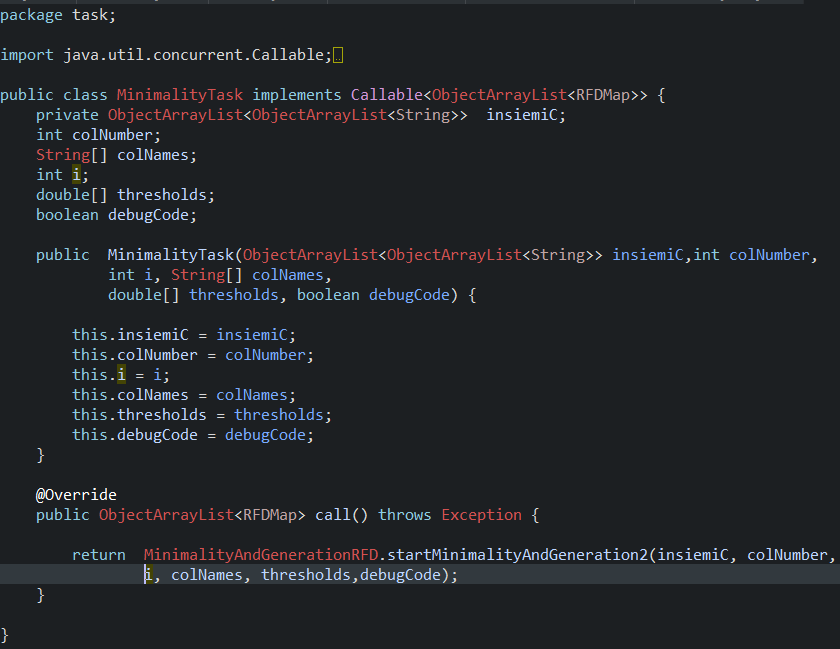
\includegraphics[scale=0.85]{Immagini/MinimalityTask.PNG}
	\caption{Minimality Task}
	\label{fig:Minimality Task}
\end{figure}




